\documentclass[a4paper, oneside]{memoir}
\usepackage[utf8]{inputenc}
\usepackage[T1]{fontenc}
\usepackage{pifont}
\usepackage{amssymb}
\usepackage{fourier}
\usepackage[dvipsnames]{xcolor}
\usepackage{tikz}
\usepackage{pdfpages}
\usepackage[sfdefault]{roboto}
\usepackage{color}

% Styles
\tikzstyle{teamshare} = [below, text width=5.4cm, inner sep = 0.5cm, text=white, align=center]
\tikzstyle{cardtext} = [below, text width=5.9cm, inner sep = 0.25cm, text centered]
\setlrmarginsandblock{0.9cm}{*}{1}
\setulmarginsandblock{1.49cm}{*}{1}
\checkandfixthelayout[nearest]
\pagestyle{empty}

% Define Commands
\newcommand{\condition}[1]{\textbf{#1}}
\newcommand{\character}[1]{\textbf{#1}}
\newdimen\titlespacing
\titlespacing=0.15cm

% Define Seperators
\newcommand{\seperator}[1]{\\ \vspace{\titlespacing} \hrulefill {} \tiny \bfseries #1 \normalfont \normalsize \hrulefill \\ \vspace{\titlespacing}}
\newcommand{\seperatoraction}{\seperator{POWER}}
\newcommand{\seperatordescription}{\seperator{DESCRIPTION}}
\newcommand{\seperatorcondition}{\seperator{CONDITION}}
\newcommand{\seperatorwin}{\seperator{HOW TO WIN}}
\newcommand{\redwinsection}{
	\seperatorwin
	\small You win if \character{President} gains the \condition{dead} condition due to the \character{Bomber} exploading.
}
\newcommand{\bluewinsection}{
	\seperatorwin
	\small You win if \character{President} does not gain the \condition{dead} condition due to the \character{Bomber} exploading.
}
\newcommand{\titlefrom}[1]{\\ \tiny > from #1 <\normalsize}

% Begin Document
\begin{document}
	
% New Page
\noindent 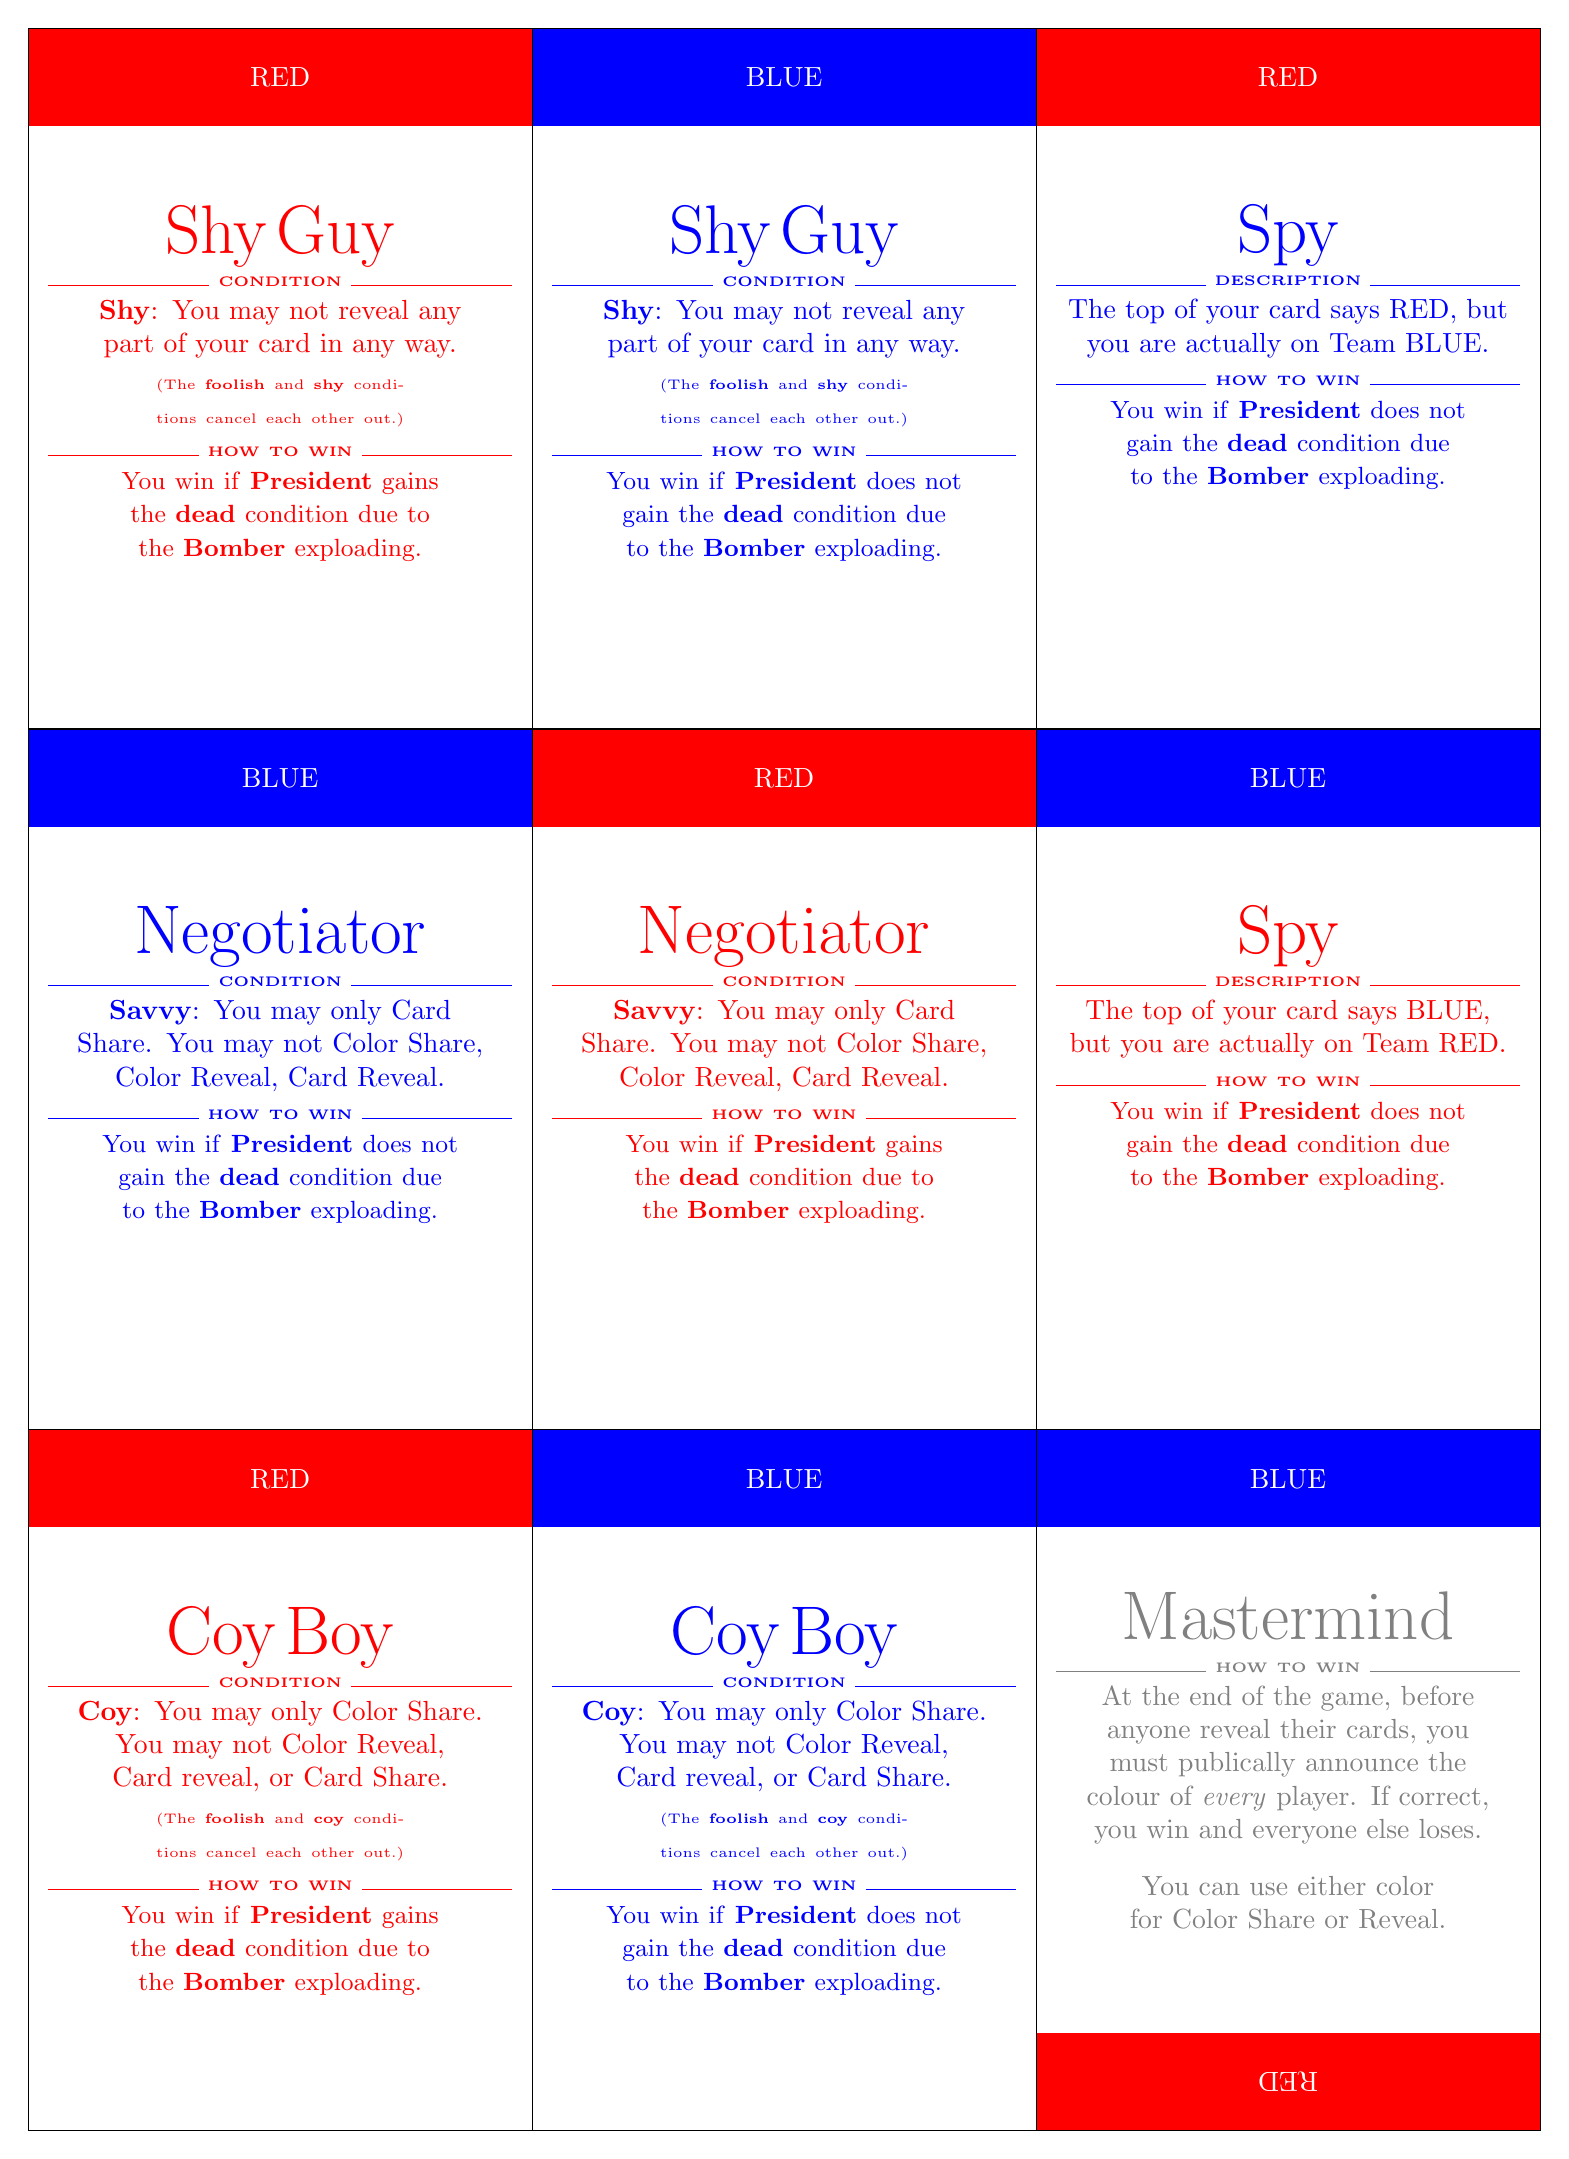
\begin{tikzpicture}[outer sep=0]

% SHY GUY (RED TEAM)
\node[teamshare, fill=red] (1) at (3.2,26.7) {\HUGE RED};
\node[cardtext, text=red] at (3.2,24.7) {
	{\Huge Shy Guy}
	\seperatorcondition
	\condition{Shy}: You may not reveal any part of your card in any way.
	\\\vspace{0.05cm}
	\tiny (The \condition{foolish} and \condition{shy} conditions cancel each other out.) \normalsize
	\redwinsection
};

% SHY GUY (BLUE TEAM)
\node[teamshare, fill=blue] at (9.6,26.7) {\HUGE BLUE};
\node[cardtext, text=blue] at (9.6,24.7) {
	{\Huge Shy Guy}
	\seperatorcondition
	\condition{Shy}: You may not reveal any part of your card in any way.
	\\\vspace{0.05cm}
	\tiny (The \condition{foolish} and \condition{shy} conditions cancel each other out.) \normalsize
	\bluewinsection
};

% SPY (BLUE TEAM)
\node[teamshare, fill=red] at (16,26.7) {\HUGE RED};
\node[cardtext, text=blue] at (16,24.7) {
	{\Huge Spy}
	\seperatordescription
	The top of your card says RED, but you are actually on Team BLUE.
	\bluewinsection
};

% NEGOTIATOR (BLUE TEAM)
\node[teamshare, fill=blue] at (3.2,17.8) {\HUGE BLUE};
\node[cardtext, text=blue] at (3.2,15.8) {
	{\Huge Negotiator}
	\seperatorcondition
	\condition{Savvy}: You may only Card Share. You may not Color Share, Color Reveal, Card Reveal.
	\bluewinsection
};

% NEGOTIATOR (RED TEAM)
\node[teamshare, fill=red] at (9.6,17.8) {\HUGE RED};
\node[cardtext, text=red] at (9.6,15.8) {
	{\Huge Negotiator}
	\seperatorcondition
	\condition{Savvy}: You may only Card Share. You may not Color Share, Color Reveal, Card Reveal.
	\redwinsection
};

% SPY (RED TEAM)
\node[teamshare, fill=blue] at (16,17.8) {\HUGE BLUE};
\node[cardtext, text=red] at (16,15.8) {
	{\Huge Spy}
	\seperatordescription
	The top of your card says BLUE, but you are actually on Team RED.
	\bluewinsection
};

% COY BOY (RED TEAM)
\node[teamshare, fill=red] at (3.2,8.9) {\HUGE RED};
\node[cardtext, text=red] at (3.2,6.9) {
	{\Huge Coy Boy}
	\seperatorcondition
	\condition{Coy}: You may only Color Share. You may not Color Reveal, Card reveal, or Card Share.
	\\\vspace{0.05cm}
	\tiny (The \condition{foolish} and \condition{coy} conditions cancel each other out.) \normalsize
	\redwinsection
};

% COY BOY (BLUE TEAM)
\node[teamshare, fill=blue] at (9.6,8.9) {\HUGE BLUE};
\node[cardtext, text=blue] at (9.6,6.9) {
	{\Huge Coy Boy}
	\seperatorcondition
	\condition{Coy}: You may only Color Share. You may not Color Reveal, Card reveal, or Card Share.
	\\\vspace{0.05cm}
	\tiny (The \condition{foolish} and \condition{coy} conditions cancel each other out.) \normalsize
	\bluewinsection
};

% MASTERMIND
\node[teamshare, fill=blue] at (16,8.9) {\HUGE BLUE};
\node[teamshare, fill=red,rotate=180] at (16,0) {\HUGE RED};
\node[cardtext, text=gray] at (16,7.1) {
	{\Huge Mastermind}
	\seperatorwin
	At the end of the game, before anyone reveal their cards, you must publically announce the colour of \emph{every} player. If correct, you win and everyone else loses.
	\\\vspace{0.3cm}
	You can use either color for Color Share or Reveal.
};

\draw (0,0) -- (19.2,0);
\draw (0,8.9) -- (19.2,8.9);
\draw (0,17.8) -- (19.2,17.8);
\draw (0,26.7) -- (19.2,26.7);

\draw (0,0) -- (0,26.7);
\draw (6.4,0) -- (6.4,26.7);
\draw (12.8,0) -- (12.8,26.7);
\draw (19.2,0) -- (19.2,26.7);



\end{tikzpicture}

%Background is not my own. But courtesy of a user on BGG
\includepdf[pages={1}, angle=90]{cardsbackground.pdf}
\pagebreak





\noindent 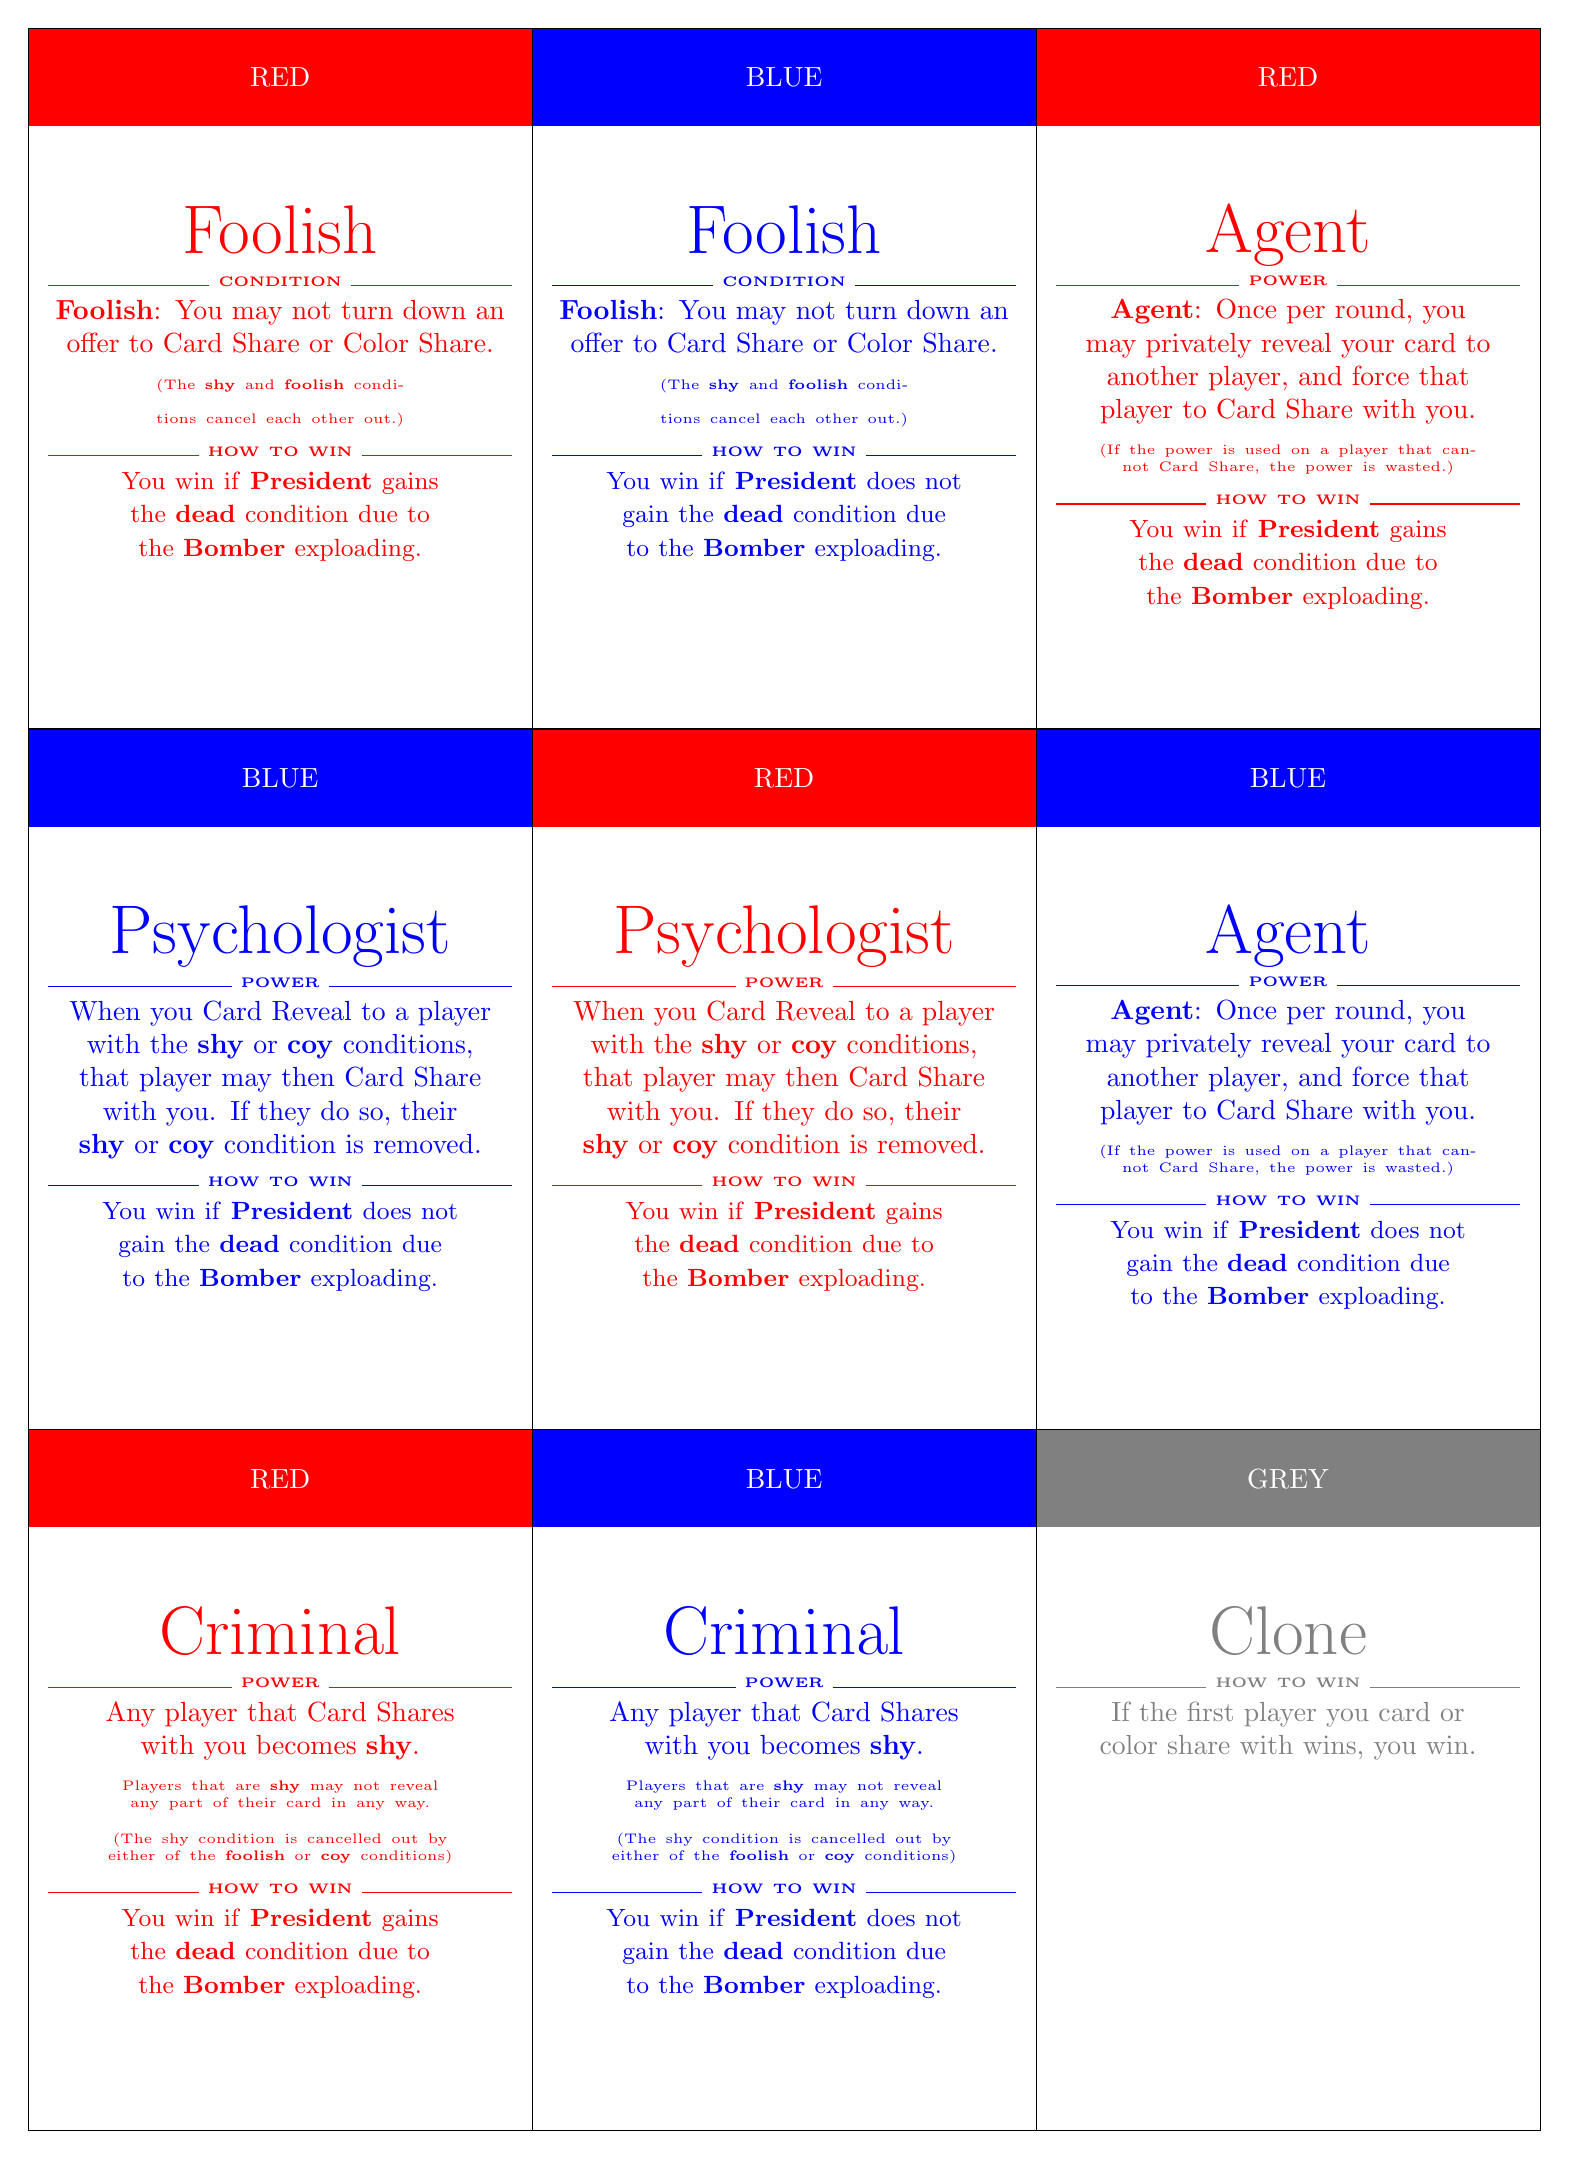
\begin{tikzpicture}[outer sep=0]

% FOOLISH (Green Team)
\node[teamshare, fill=red] (1) at (3.2,26.7) {\HUGE RED};
\node[cardtext, text=red] at (3.2,24.7) {
	{\Huge Foolish}
	\seperatorcondition
	\condition{Foolish}: You may not turn down an offer to Card Share or Color Share.
	\\\vspace{0.05cm}
	\tiny (The \condition{shy} and \condition{foolish} conditions cancel each other out.) \normalsize
	\redwinsection
};

% FOOLISH (BLUE TEAM)
\node[teamshare, fill=blue] at (9.6,26.7) {\HUGE BLUE};
\node[cardtext, text=blue] at (9.6,24.7) {
	{\Huge Foolish}
	\seperatorcondition
	\condition{Foolish}: You may not turn down an offer to Card Share or Color Share.
	\\\vspace{0.05cm}
	\tiny (The \condition{shy} and \condition{foolish} conditions cancel each other out.) \normalsize
	\bluewinsection
};

% AGENT (RED TEAM)
\node[teamshare, fill=red] at (16,26.7) {\HUGE RED};
\node[cardtext, text=red] at (16,24.7) {
	{\Huge Agent}
	\seperatoraction
	\condition{Agent}: Once per round, you may privately reveal your card to \\another player, and force that player to Card Share with you.
	\\\vspace{0.25cm}
	\tiny (If the power is used on a player that cannot Card Share, the power is wasted.)
	\redwinsection
};

% PSYCHOLOGIST (BLUE TEAM)
\node[teamshare, fill=blue] at (3.2,17.8) {\HUGE BLUE};
\node[cardtext, text=blue] at (3.2,15.8) {
	{\Huge Psychologist}
	\seperatoraction
	When you Card Reveal to a player with the \condition{shy} or \condition{coy} conditions, that player may then Card Share with you. If they do so, their \condition{shy} or \condition{coy} condition is removed.
	\bluewinsection
};

% PSYCHOLOGIST (RED TEAM)
\node[teamshare, fill=red] at (9.6,17.8) {\HUGE RED};
\node[cardtext, text=red] at (9.6,15.8) {
	{\Huge Psychologist}
	\seperatoraction
	When you Card Reveal to a player with the \condition{shy} or \condition{coy} conditions, that player may then Card Share with you. If they do so, their \condition{shy} or \condition{coy} condition is removed.
	\redwinsection
};

% AGENT (BLUE TEAM)
\node[teamshare, fill=blue] at (16,17.8) {\HUGE BLUE};
\node[cardtext, text=blue] at (16,15.8) {
	{\Huge Agent}
	\seperatoraction
	\condition{Agent}: Once per round, you may privately reveal your card to \\another player, and force that player to Card Share with you.
	\\\vspace{0.25cm}
	\tiny (If the power is used on a player that cannot Card Share, the power is wasted.)
	\bluewinsection
};

% CRIMINAL (RED TEAM)
\node[teamshare, fill=red] at (3.2,8.9) {\HUGE RED};
\node[cardtext, text=red] at (3.2,6.9) {
	{\Huge Criminal}
	\seperatoraction
	Any player that Card Shares with you becomes \condition{shy}.
	\\\vspace{0.25cm}
	\tiny Players that are \condition{shy} may not reveal any part of their card in any way.
	\\\vspace{0.25cm}
	\tiny (The shy condition is cancelled out by \\either of the \condition{foolish} or \condition{coy} conditions)
	\redwinsection
};

% CRIMINAL (BLUE TEAM)
\node[teamshare, fill=blue] at (9.6,8.9) {\HUGE BLUE};
\node[cardtext, text=blue] at (9.6,6.9) {
	{\Huge Criminal}
	\seperatoraction
	Any player that Card Shares with you becomes \condition{shy}.
	\\\vspace{0.25cm}
	\tiny Players that are \condition{shy} may not reveal any part of their card in any way.
	\\\vspace{0.25cm}
	\tiny (The shy condition is cancelled out by \\either of the \condition{foolish} or \condition{coy} conditions)
	\bluewinsection
};

% CLONE
\node[teamshare, fill=gray] at (16,8.9) {\HUGE GREY};
\node[cardtext, text=gray] at (16,6.9) {
	{\Huge Clone}
	\seperatorwin
	If the first player you card or color share with wins, you win.
};

\draw (0,0) -- (19.2,0);
\draw (0,8.9) -- (19.2,8.9);
\draw (0,17.8) -- (19.2,17.8);
\draw (0,26.7) -- (19.2,26.7);

\draw (0,0) -- (0,26.7);
\draw (6.4,0) -- (6.4,26.7);
\draw (12.8,0) -- (12.8,26.7);
\draw (19.2,0) -- (19.2,26.7);



\end{tikzpicture}

%Background is not my own. But courtesy of a user on BGG
\includepdf[pages={1}, angle=90]{cardsbackground.pdf}







\noindent 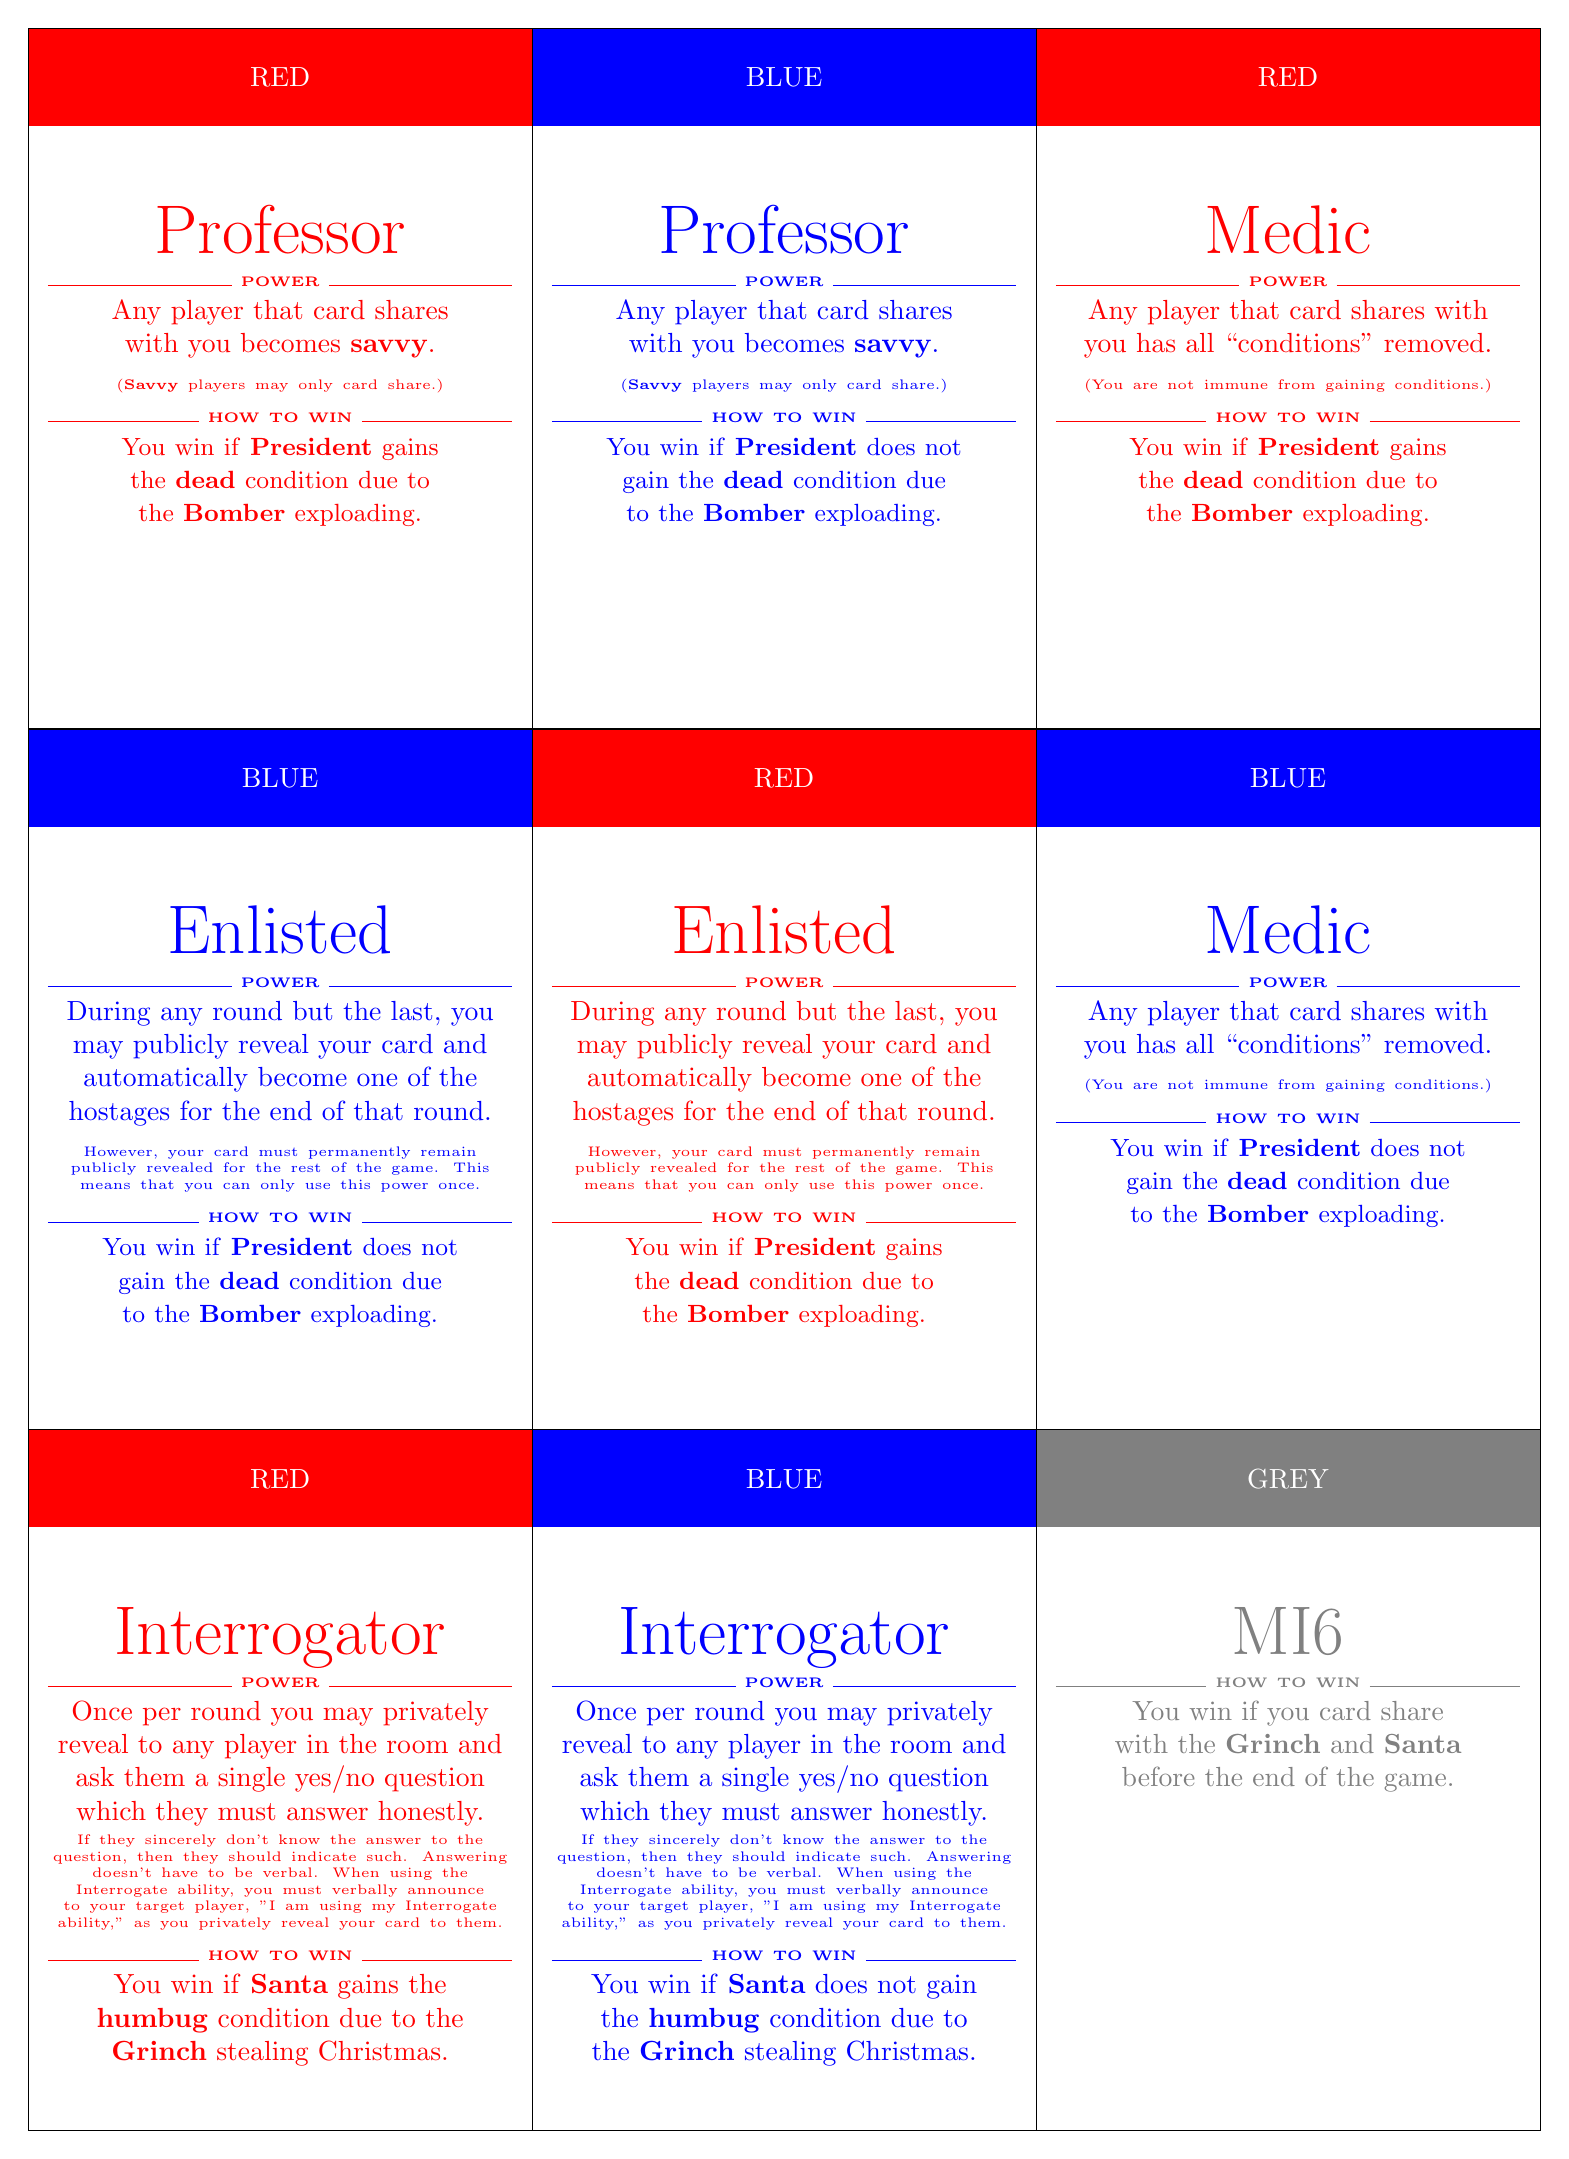
\begin{tikzpicture}[outer sep=0]

% PROFESSOR (RED TEAM)
\node[teamshare, fill=red] (1) at (3.2,26.7) {\HUGE RED};
\node[cardtext, text=red] at (3.2,24.7) {
	{\Huge Professor}
	\seperatoraction
	Any player that card shares with you becomes \condition{savvy}.
	\\\vspace{0.25cm}
	\tiny (\condition{Savvy} players may only card share.)
	\redwinsection
};

% PROFESSOR (BLUE TEAM)
\node[teamshare, fill=blue] at (9.6,26.7) {\HUGE BLUE};
\node[cardtext, text=blue] at (9.6,24.7) {
	{\Huge Professor}
	\seperatoraction
	Any player that card shares with you becomes \condition{savvy}.
	\\\vspace{0.25cm}
	\tiny (\condition{Savvy} players may only card share.)
	\bluewinsection
};

% MEDIC (BLUE TEAM)
\node[teamshare, fill=red] at (16,26.7) {\HUGE RED};
\node[cardtext, text=red] at (16,24.7) {
	{\Huge Medic}
	\seperatoraction
	Any player that card shares with you has all “conditions” removed.
	\\\vspace{0.25cm}
	\tiny (You are not immune from gaining conditions.)
	\redwinsection
};

% ENLISTED (BLUE TEAM)
\node[teamshare, fill=blue] at (3.2,17.8) {\HUGE BLUE};
\node[cardtext, text=blue] at (3.2,15.8) {
	{\Huge Enlisted}
	\seperatoraction
	During any round but the last, you may publicly reveal your card and automatically become one of the hostages for the end of that round. 
	\\\vspace{0.25cm}
	\tiny However, your card must permanently remain publicly revealed for the rest of the game. This means that you can only use this power once.
	\bluewinsection
};

% ENLISTED (RED TEAM)
\node[teamshare, fill=red] at (9.6,17.8) {\HUGE RED};
\node[cardtext, text=red] at (9.6,15.8) {
	{\Huge Enlisted}
	\seperatoraction
	During any round but the last, you may publicly reveal your card and automatically become one of the hostages for the end of that round. 
	\\\vspace{0.25cm}
	\tiny However, your card must permanently remain publicly revealed for the rest of the game. This means that you can only use this power once.
	\redwinsection
};

% MEDIC (BLUE TEAM)
\node[teamshare, fill=blue] at (16,17.8) {\HUGE BLUE};
\node[cardtext, text=blue] at (16,15.8) {
	{\Huge Medic}
	\seperatoraction
	Any player that card shares with you has all “conditions” removed.
	\\\vspace{0.25cm}
	\tiny (You are not immune from gaining conditions.)
	\bluewinsection
};

% INTERROGATOR (RED TEAM)
\node[teamshare, fill=red] at (3.2,8.9) {\HUGE RED};
\node[cardtext, text=red] at (3.2,6.9) {
	{\Huge Interrogator}
	\seperatoraction
	Once per round you may privately \\
	reveal to any player in the room and \\
	ask them a single yes/no question \\
	which they must answer honestly. \\
	\vspace{0.1cm} 
	\tiny
	If they sincerely don’t know the answer to the question, then they should indicate such. Answering \\
	doesn’t have to be verbal. When using the \\
	Interrogate ability, you must verbally announce to your target player, "I am using my Interrogate ability," as you privately reveal your card to them.
	\seperatorwin
	\normalsize You win if \character{Santa} gains the \condition{humbug} condition due to the \character{Grinch} stealing Christmas.
};

% INTERROGATOR (BLUE TEAM)
\node[teamshare, fill=blue] at (9.6,8.9) {\HUGE BLUE};
\node[cardtext, text=blue] at (9.6,6.9) {
	{\Huge Interrogator}
	\seperatoraction
	Once per round you may privately \\
	reveal to any player in the room and \\
	ask them a single yes/no question \\
	which they must answer honestly. \\
	\vspace{0.1cm} 
	\tiny
	If they sincerely don’t know the answer to the question, then they should indicate such. Answering \\
	doesn’t have to be verbal. When using the \\
	Interrogate ability, you must verbally announce to your target player, "I am using my Interrogate ability," as you privately reveal your card to them.
	\seperatorwin
	\normalsize You win if \character{Santa} does not gain the \condition{humbug} condition due to the \character{Grinch} stealing Christmas.
};

% MI6
\node[teamshare, fill=gray] at (16,8.9) {\HUGE GREY};
\node[cardtext, text=gray] at (16,6.9) {
	{\Huge MI6}
	\seperatorwin
	You win if you card share with the \character{Grinch} and \character{Santa} before the end of the game.
};

\draw (0,0) -- (19.2,0);
\draw (0,8.9) -- (19.2,8.9);
\draw (0,17.8) -- (19.2,17.8);
\draw (0,26.7) -- (19.2,26.7);

\draw (0,0) -- (0,26.7);
\draw (6.4,0) -- (6.4,26.7);
\draw (12.8,0) -- (12.8,26.7);
\draw (19.2,0) -- (19.2,26.7);



\end{tikzpicture}

%Background is not my own. But courtesy of a user on BGG
\includepdf[pages={1}, angle=90]{cardsbackground.pdf}
\pagebreak


\end{document}
